\documentclass[a4paper,10pt]{article}
\usepackage[utf8]{inputenc}
\usepackage{graphicx}
\usepackage{courier} %% Sets font for listing as Courier.
\usepackage{listings, xcolor}
\lstset{
tabsize = 4, %% set tab space width
showstringspaces = false, %% prevent space marking in strings, string is defined as the text that is generally printed directly to the console
numbers = left, %% display line numbers on the left
commentstyle = \color{green}, %% set comment color
keywordstyle = \color{blue}, %% set keyword color
stringstyle = \color{red}, %% set string color
rulecolor = \color{black}, %% set frame color to avoid being affected by text color
basicstyle = \small \ttfamily , %% set listing font and size
breaklines = true, %% enable line breaking
numberstyle = \tiny,
}
%opening
\title{Relatório TP1 SBS-MLFA}
\author{Luis Freitas - PG38347; Daniel Pereira}

\begin{document}

\maketitle

\begin{abstract}

\end{abstract}

\section{Introdução}
\newpage
\section{Metodologias}
\subsection{CRISP-DM}
\subsection{Modelo Baseados em Árvores}
\newpage



\section{Arquiteturas e Ferramentas}
\newpage

\section{DataSet da Competição}

\newpage


\subsection{Contexto do Dataset}
%escrever por palavras nossas
O dataset utilizado neste projeto é referente ao nível de incidentes rodoviários na zona de Braga e contém algumas features que representam a magnitude do atraso que se verifica a cada hora, a temperatura, a pressão atmosférica, a velocidade do vento e ainda outras features. 

O principal objetivo é aprimorar um modelo de Machine Learning Baseado em Arvores mas também fazer uma analise exploratoria completa dos dados para se retirar algumas informações importantes do dataset. Outo ponto passa por conseguir preprarar o dataset com técnicas de engenharia de dados para se obter os melhores resultados possiveis. Este dataset é referente a uma competição da plataforma Kaggle

Em relação as features do dataset estas são apresentadas da seguinte forma:

\begin{enumerate}
	\item \textbf{city\underline{ }name} - nome da cidade em causa;
	\item \textbf{record\underline{ }date} - o timestamp associado ao registo
	\item \textbf{magnitude\underline{ }of\underline{ }delay} - magnitude do atraso provocado pelos incidentes que se verificam no record\underline{ }date correspondente;
	\item \textbf{delay\underline{ }in\underline{ }seconds}  -  atraso, em segundos, provocado pelos incidentes que se verificam no record\underline{ }date correspondente;
	\item \textbf{affected\underline{ }roads} - estradas afectadas pelos incidentes que se verificam no record\underline{ }date correspondente;
	\item \textbf{luminosity} - o nível de luminosidade que se verificava na cidade de Braga;
	\item \textbf{avg\underline{ }temperature} - valor médio da temperatura para o record\underline{ }date na cidade de Braga;
	\item \textbf{avg\underline{ }atm\underline{ }pressure} - valor médio da pressão atmosférica para o record\underline{ }date na cidade de Braga;
	\item \textbf{avg\underline{ }humidity} - valor médio da humidade para o record\underline{ }date na cidade de Braga;
	\item \textbf{avg\underline{ }wind\underline{ }speed} - valor médio da velocidade do vento para o record\underline{ }date na cidade de Braga;
	\item \textbf{avg\underline{ }precipitation} - valor médio de precipitação para o record\underline{ }date na cidade de Braga;
	\item \textbf{avg\underline{ }rain} - avaliação qualitativa do nível de precipitação para o record\underline{ }date na cidade de Braga;
	\item \textbf{accidents} - indicação acerca do nível de incidentes rodoviários que se verificam no record\underline{ }date correspondente na cidade de Braga;
\end{enumerate}

\newpage

\subsection{Análise e Transformação dos Dados}

O DataSet utilizado apresenta cinco mil linhas e foi analisado de forma a serem retiradas informações que pudessem ser uteis no desenvolvimento do modelo. 
 

(DANIEL ESCREVE AQUI A ANÁLISE DE DADOS QUE JUSTIFIQUE TODAS AS TRANSFORMAÇÕES FEITAS)

\begin{figure} [ h! ]
  \centering
  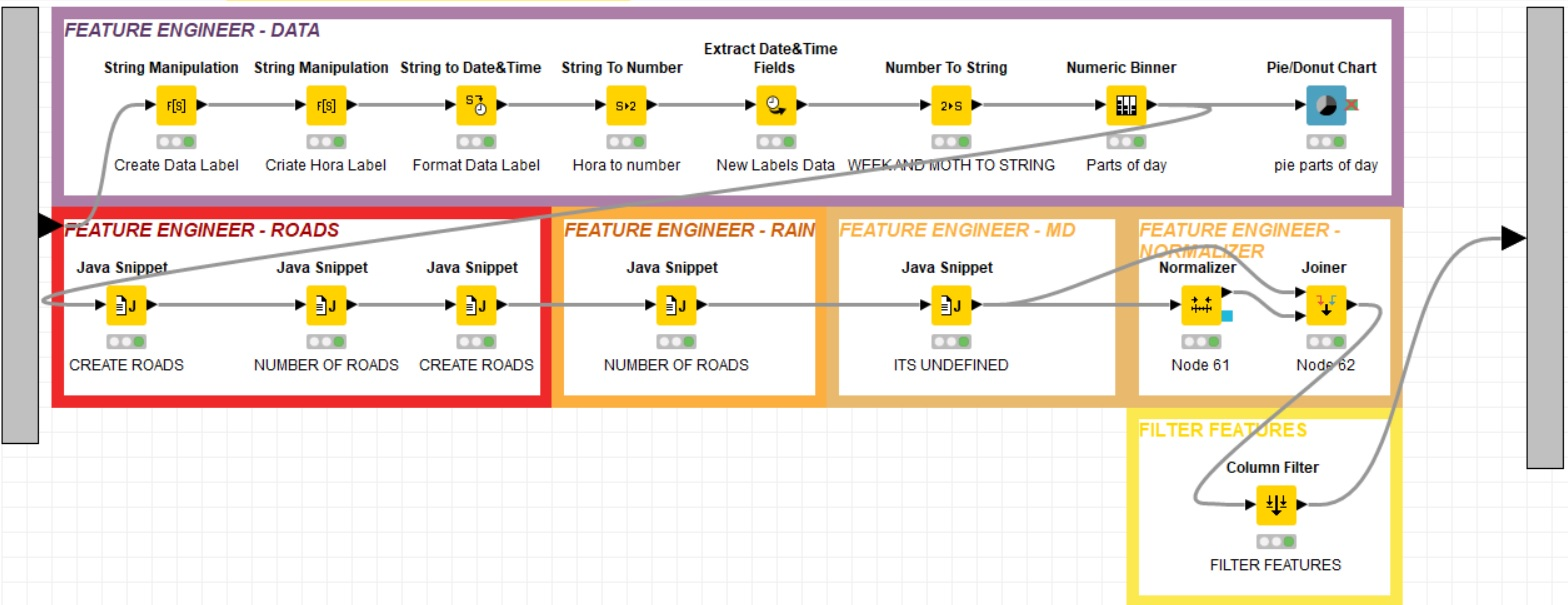
\includegraphics[width=\linewidth]{imagens/DATAPREPARATION.jpg}
  \caption{Workflow Data Preparation}
  \label{fig:DATAPREPARATION}
\end{figure}

As transformações de dados realizadas foram uteis para os resultados do modelo e foram suportadas pela analise de dados efetuada e explicada no capitulo anterior. 


Como se pode ver na figura em baixo, pode-se retirar várias informações de algumas features, como por exemplo da record\underline{ }date e da affected\underline{ }roads. Nesta forma inicial estas duas features não contém muita informação pertinente para o modelo. 

\begin{figure} [ h! ]
  \centering
  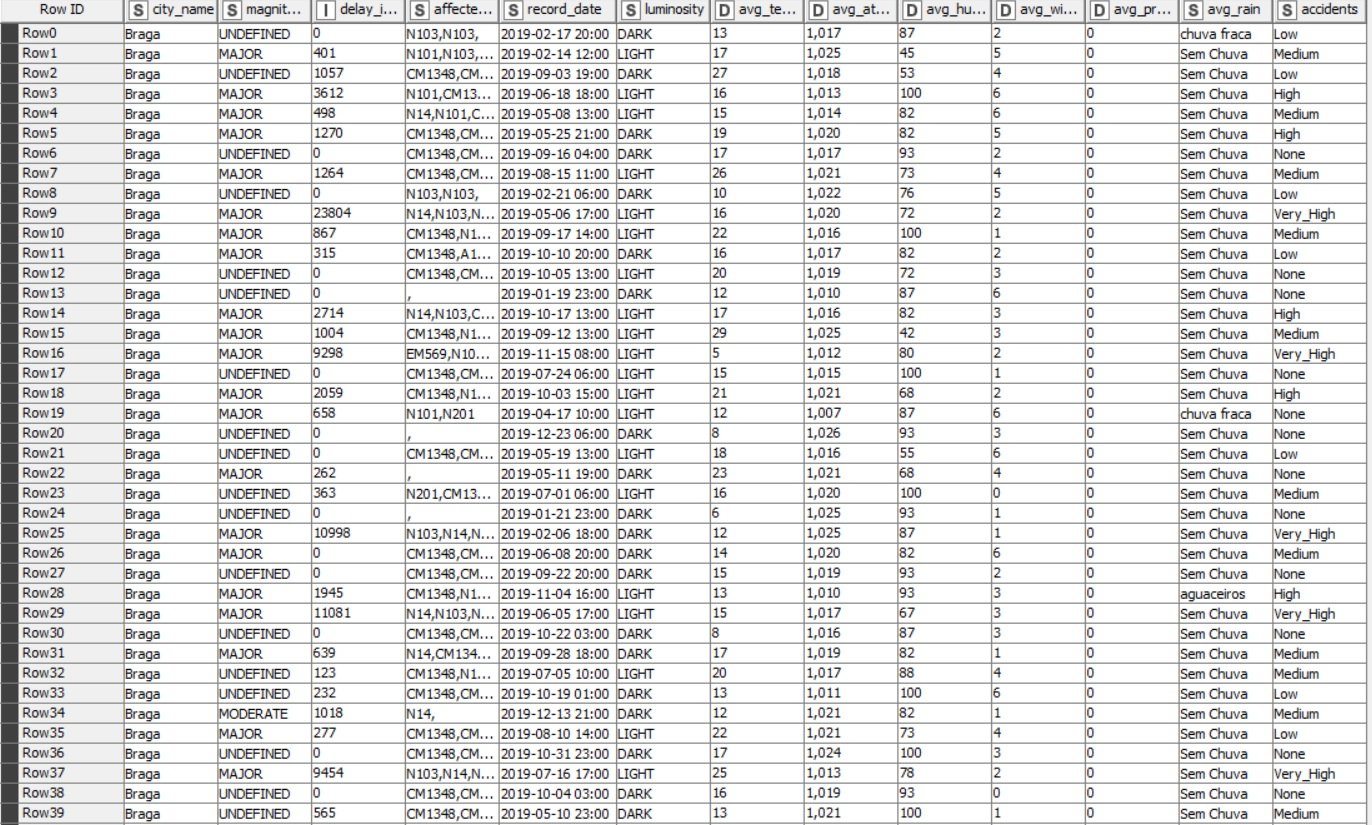
\includegraphics[width=\linewidth]{imagens/DATASET.jpg}
  \caption{Data Set}
  \label{fig:DATASET}
\end{figure}

A partir de técnicas de tratamento de dados foi possivel criar novas features geradas a partir de informação disponivel na feature record\underline{ }date, foi separada a data da hora em duas novas features, foi criada a nova coluna do trimestre e das semans, assim como o dia da semana e a parte do dia. 

\begin{figure} [ h! ]
  \centering
  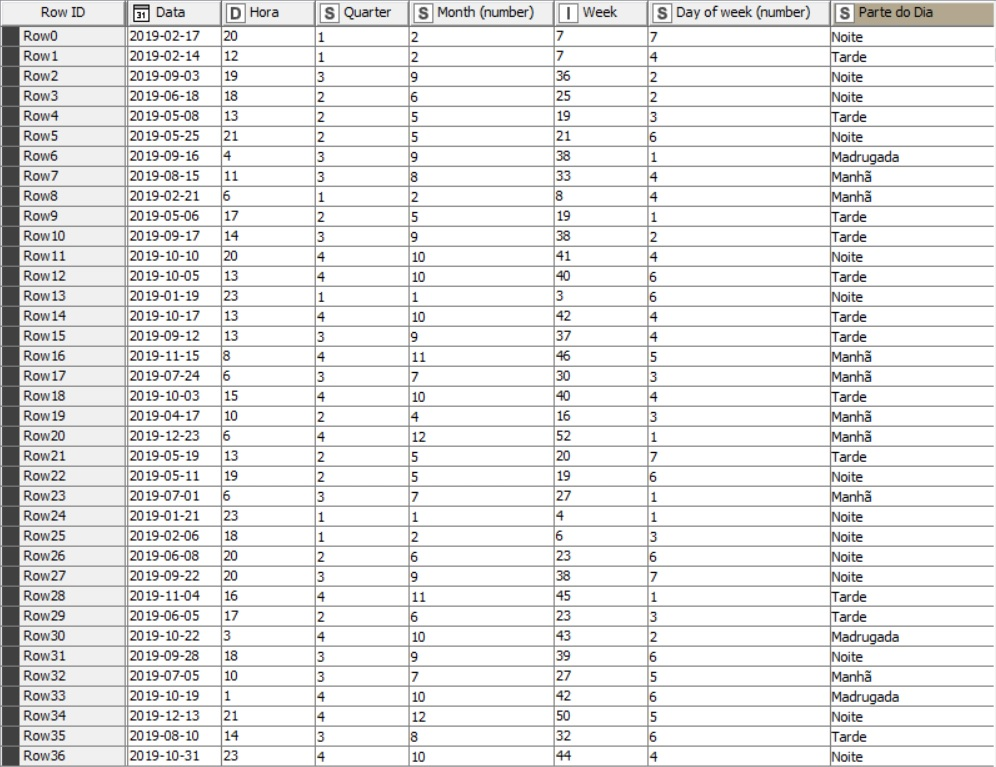
\includegraphics[width=\linewidth]{imagens/DATAFE.jpg}
  \caption{Novas Features geradas da \textbf{record\underline{ }date}}
  \label{fig:DATAFE}
\end{figure}
\newpage
A feature \textbf{Parte do Dia} foi concebida a partir da \textbf{Hora} e foram selecionados intervalos de forma a que cada parte do dia ficasse com frequencias identicas. 

\begin{figure} [ h! ]
  \centering
  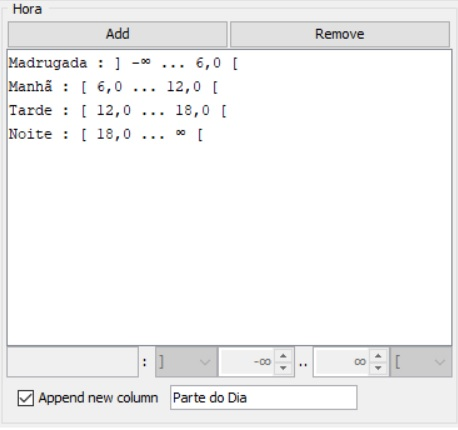
\includegraphics[width=0.5\linewidth]{imagens/partedodiacode.jpg}
  \caption{Configuração da Feature \textbf{Parte do Dia}}
  \label{fig:partedodiacode}
\end{figure}

\begin{figure} [ h! ]
 \centering
  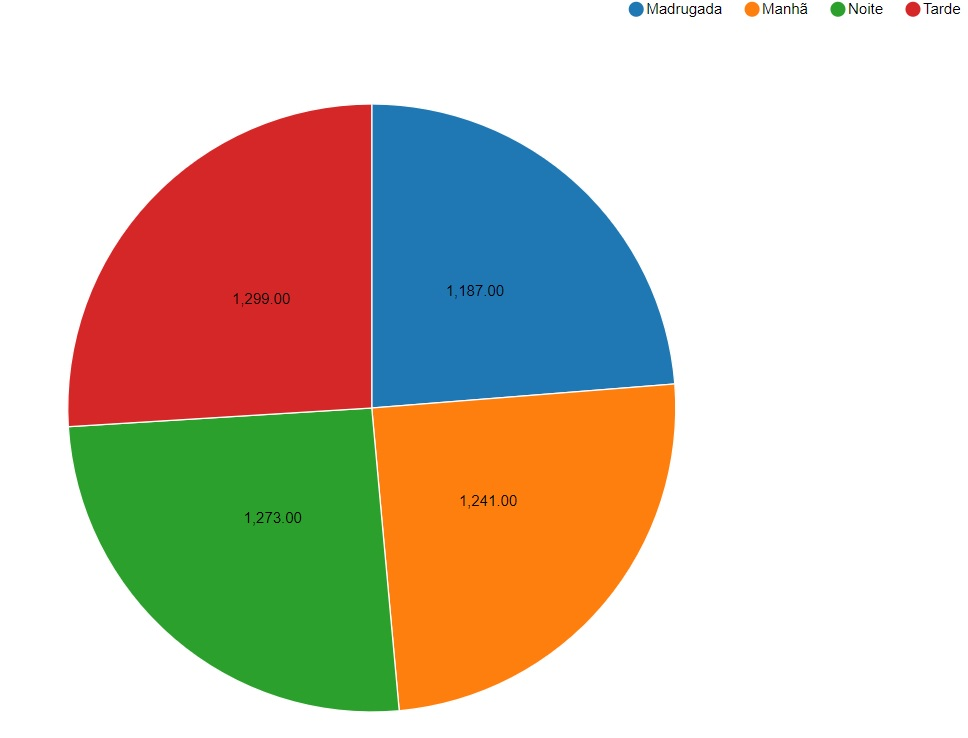
\includegraphics[width=0.9\linewidth,scale=1.2]{imagens/partedodiafreq.jpg}
  \caption{Distribuição da Feature \textbf{Parte do Dia}}
  \label{fig:partedodiafreq}
\end{figure}

Outra das transformações mais importantes foi sobre a feature \textbf{affected\underline{ }roads}, em baixo podemos ver as novas colunas geradas pelas transformações de dados nessa feature. 

\begin{figure} [ h! ]
  \centering
  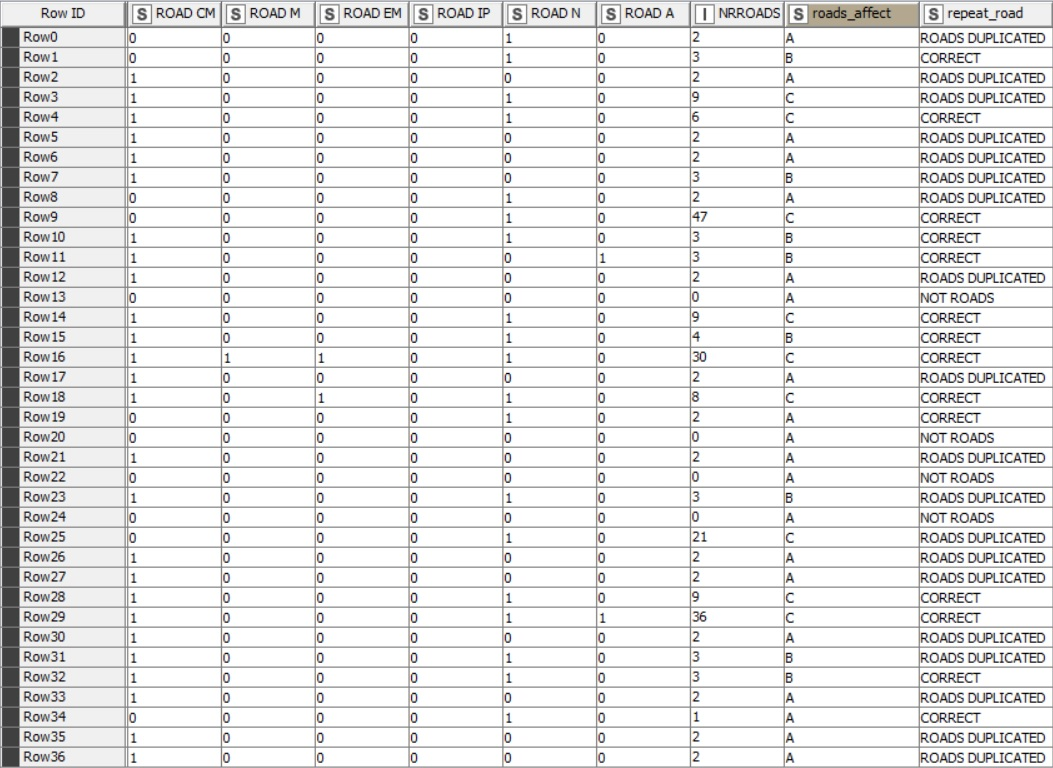
\includegraphics[width=0.9\linewidth,scale=1.2]{imagens/roads.jpg}
  \caption{Novas Features geradas a partir da }
  \label{fig:roads}
\end{figure}

Como se pode ver, as features ROAD CM, ROAD M, ROAD EM, ROAD IP, ROAD N e ROAD A representam o tipo de estrada. Se a estrada daquele tipo estiver afetada no acidente, o valor dessa feature vai ser "1", caso não esteja, vai ser "0", por exemplo, na "Row 2" a coluna "ROAD N" tem valor "1", logo, estradas do tipo "N" estão afetadas pelo acidente. 
A feature "NROADS" representa o número de estradas afetadas pelos acidentes, está variavel tem muita importancia no modelo gerado porque se houver um grande número de estradas é quase certo que o acidente é grave, este valor é justificado com a seguinte caixa de bigodes. 

\begin{figure} [ h! ]
  \centering
  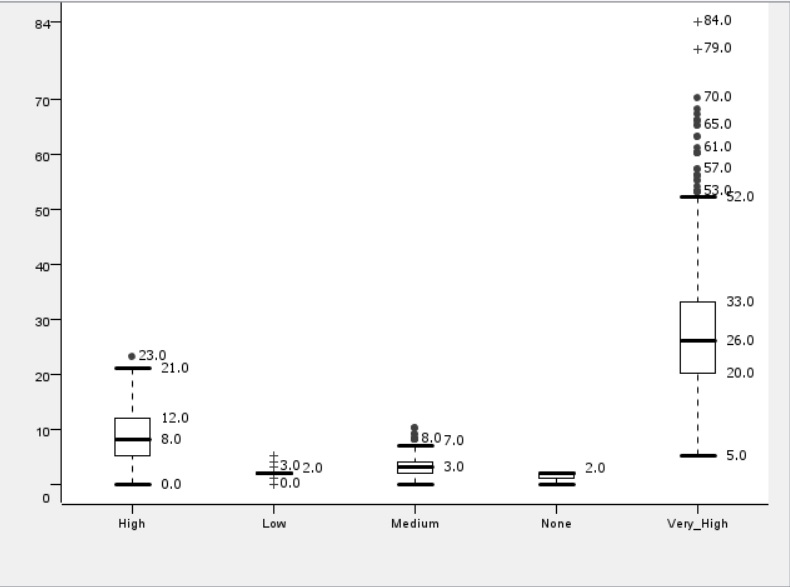
\includegraphics[width=0.9\linewidth,scale=1.2]{imagens/bproads.jpg}
  \caption{Box Plot NRROADS vs Count(accuracy) }
  \label{fig:bproads}
\end{figure}

A feature "roads\underline{ }affect" é usada para categorizar a feature "NRROADS". É claro que se ambas estas features entrarem no modelo este terá problemas de multicolineariadade, mas foram as duas geradas para se perceber qual delas funcionará melhior no modelo. A feature conta com a categoria "A","B" e "C" e é dividida da seguinte forma: 

\begin{lstlisting}[language = Java , frame = trBL , firstnumber = last , escapeinside={(*@}{@*)}]
String[] parts = c_affected_roads.split(",");		
out_NRROADS = parts.length;
 
if (out_NRROADS >= 3 && out_NRROADS < 6 ){
	out_roads_affect = "B";
}else if (out_NRROADS >= 6){
	out_roads_affect = "C";
}else {
	out_roads_affect = "A";
}
\end{lstlisting}
Finalmente, a última feature a ser gerada ("repeat\underline{ }road") revela se na feature das "roads\underline{ }affect" existem estradas repetidas, não esxistem estradas, ou simplesmente existem estradas mas não repetidas. 

Foram efetuadas mais algumas transformações, das quais categorizar, de uma forma diferente,  a feature "avg\underline{ }rain". Tendo o valor "0" caso a "avg\underline{ }rain" tenha o valor "Sem Chuva", e o valor "1" caso contrário.  
Foi também criada uma feature para categorizar de forma diferente a feature \textbf{magnitude\underline{ }of\underline{ }delay}, caso seja "UNDEFINED", ficará com o valor "1", e toma o valor "0" caso contrário. 

Foram acrescentadas todas as features numéricas de forma normalizada ao dataset para depois se comparar de que forma é que o modelo se comporta com algumas normalizações. 




\newpage
\subsection{Modelação}
\subsection{Análise de Resultados}



\newpage
\section{DataSet 1}
\subsection{Contexto do Dataset}
\subsection{Análise e Compreensão dos Dados}
\subsection{Modelação}
\subsection{Análise de Resultados}
\section{Conclusão}

\end{document}
